		\begin{enumerate}
			\item \begin{enumerate}
					\item Note that if $y(x)=0$, then $y(0)=0$. Simulating with initial conditions $(x_0,y_0)=(0,0)$, we see
					an approximation that is clearly not the constant zero function.
					\begin{center}
						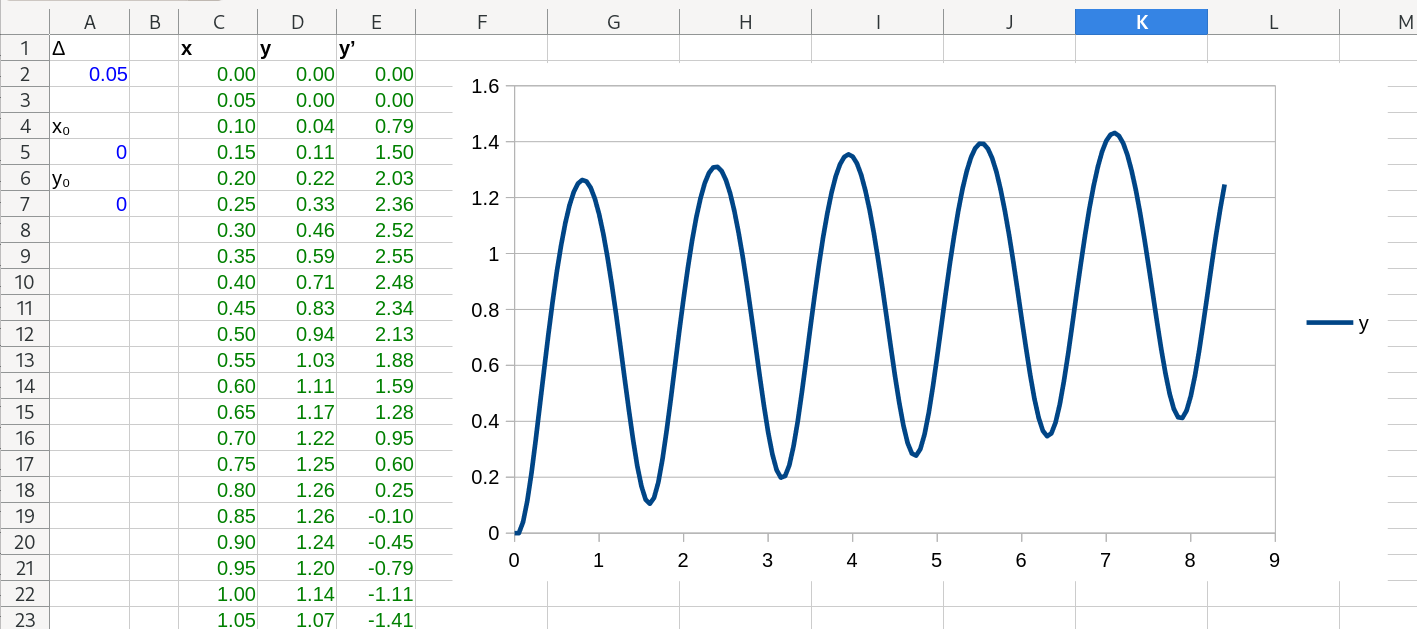
\includegraphics[height=2in]{resources/tutorial-01-sheet1.png}
					\end{center}
					
					Analytically, if $y(x)=0$, then $y'(x) = 0$ for all $x$. However, the differential equation is not the constant zero function.
					
					\item Simulating, we see that the simulated values of $y$ with $\Delta=0.7854$ are extremely tiny.
					\begin{center}
						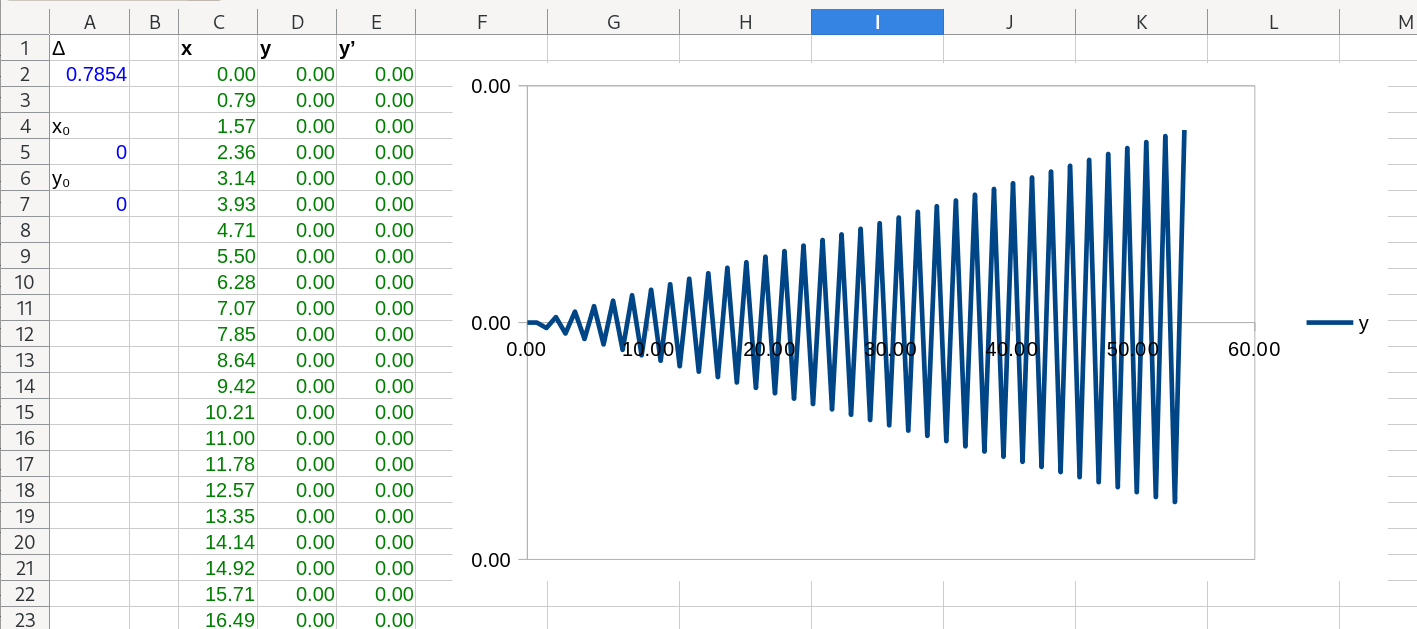
\includegraphics[height=2in]{resources/tutorial-01-sheet1b.png}
					\end{center}
					We know from simulating with other values of $\Delta$ that the values of $y$ do not stay close to zero, so using $\Delta=0.7854$ does
					not lead to a reasonable approximation.
					
					\item Simulating with $\Delta=0.1$, we can look at the data of our spreadsheet to find the local maxima.
					\begin{center}
						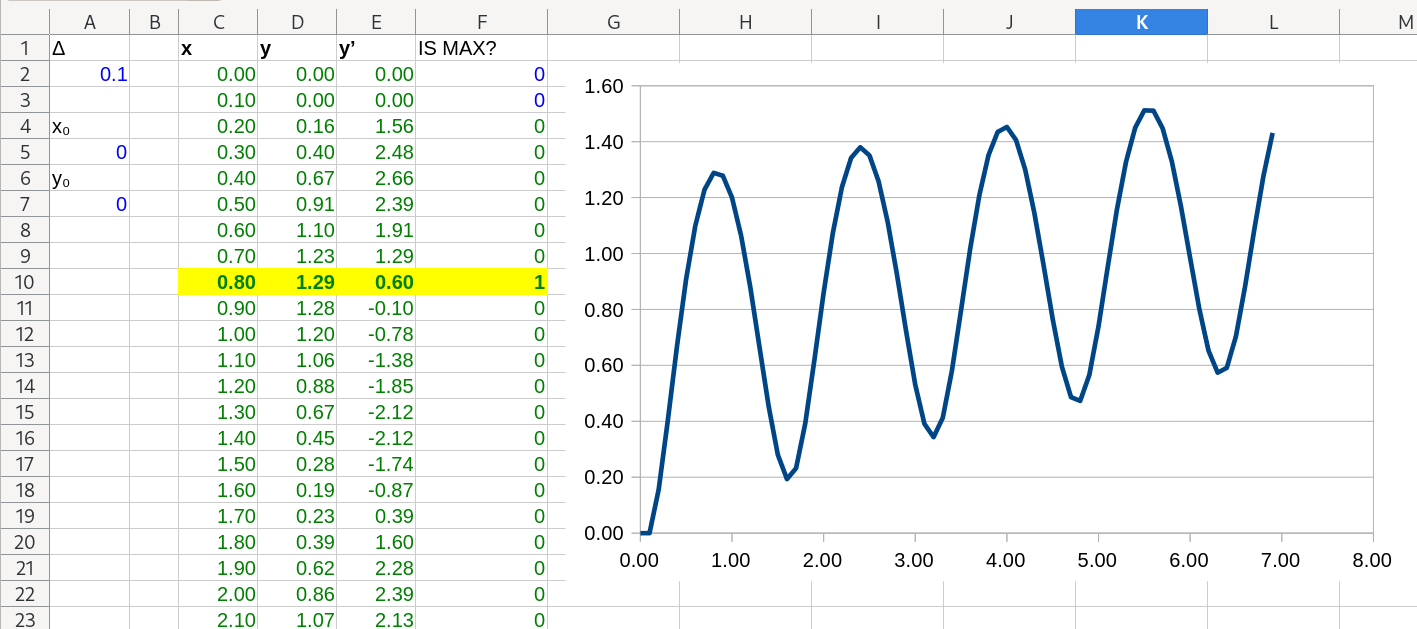
\includegraphics[height=2in]{resources/tutorial-01-sheet1c.png}
					\end{center}
					They occur at $x=0.8, 2.4, 4.0, 5.5,\ldots$.

					\item Local maxima occur when $y'=0$ and $y''\leq 0$ (note when $y''=0$, further testing is required).
					From the differential equation, we can see that $y'(x)=0$ when $x$ is a multiple of $\frac{\pi}{4}$.
					Computing the second derivative,
					\[
						y''(x) = \frac{16\cos(4x)}{1+y} - \frac{4\sin(4x)}{(1+y)^2}.
					\]
					Testing $y''$ when $x=n\frac{\pi}{4}$, we see that it is negative when $n=2k+1$, so we have local maximums at
					$x=\pi/4, 5\pi/4, 9\pi/4, 13\pi/4,\ldots\approx0.79,2.36,3.92,5.50,\ldots$, which is close to our numeric approximations
					from the previous part.

			\end{enumerate}
			\item \begin{enumerate}
					\item Making a table of values, we have

					\begin{tabular}{l|l|l|l|l}
						$\Delta$&Max 1&Max 2&Max 3 &Max 4\\
						\hline
						$0.1$    & 1.29 & 1.38 & 1.45 & 1.51 \\
						$0.05$   & 1.26 & 1.31 & 1.35 & 1.39 \\
						$0.01$   & 1.24 & 1.25 & 1.26 & 1.27 \\
						$0.005$  & 1.24 & 1.24 & 1.25 & 1.25
					\end{tabular}

					\item Numerical evidence suggests that the solutions are periodic without an upward drift. As $\Delta$ is
					made smaller and smaller, the difference in height between the first four peaks gets smaller and smaller and
					seems to converge $\sim 1.24$. Since we already know that the local maxima appear at regular intervals, this suggests
					that the peaks are not drifting and the solution as a whole is periodic.

					\item Computing, $\displaystyle A'(x) = \frac{4\sin(4x)}{\sqrt{3-2\cos(4x)}} = \frac{4\sin(4x)}{A(x)+1}$, which fits the form
					of the differential equation.

					\item $A$ is a periodic solution to the differential equation satisfying $A(0)=0$, so there must be a periodic solution to
					the differential equation.
			\end{enumerate}
			\item \begin{enumerate}
				\item Modifying the previous spreadsheet we get
					\begin{center}
						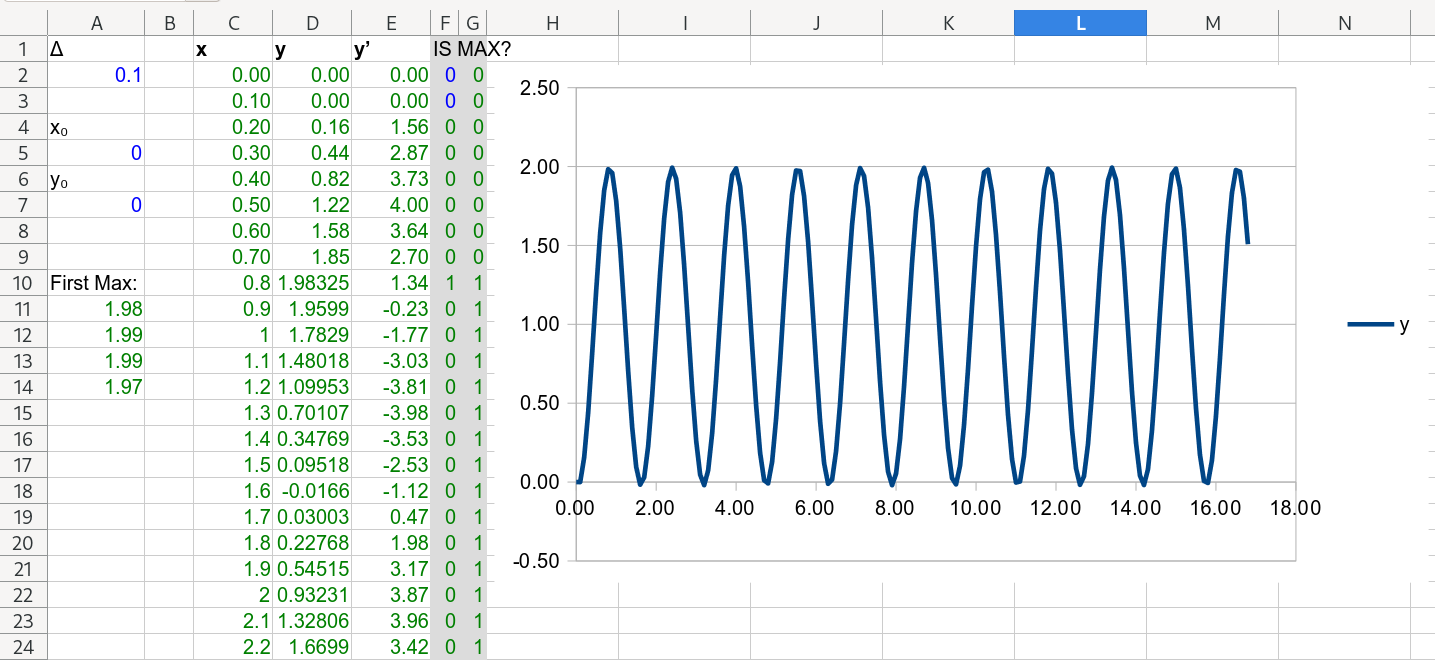
\includegraphics[height=2in]{resources/tutorial-01-sheet3a.png}
					\end{center}
				\item An exect solution satisfying $y(0)=0$ (found by integration) is $y(x)=-\cos(4x)+1$.
					Plotting, we see that the error doesn't increase much compared to $x$.
					\begin{center}
						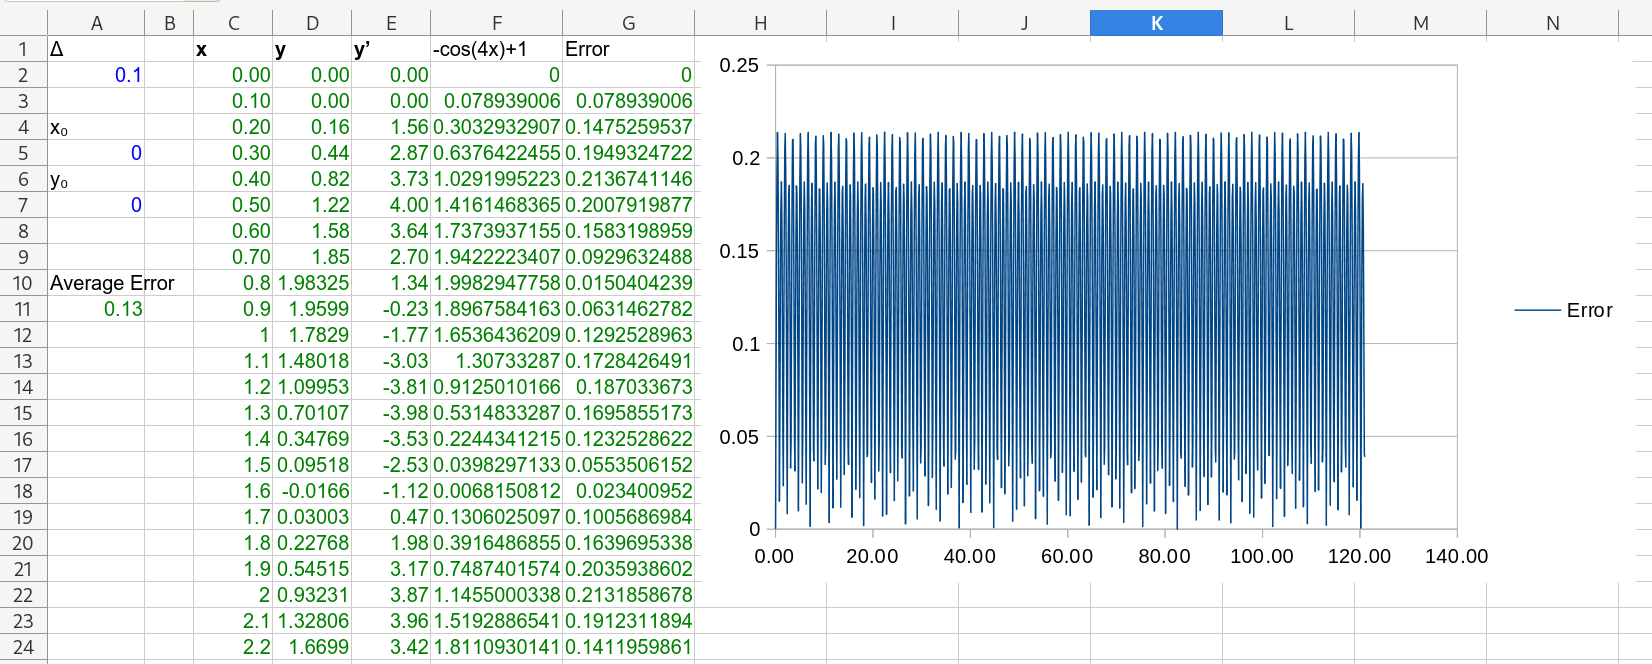
\includegraphics[height=2in]{resources/tutorial-01-sheet3b.png}
					\end{center}
				\item We have seen two cases of Euler's method producing errors. For the first differential equation, errors did accumulate, but in the second
					differential equation, errors did not end up accumulating. The conclusion is, you cannot always assume that errors end up
					accumulating when using Euler's method (you must do an analysis on a case-by-case basis)!

			\end{enumerate}
		\end{enumerate}
